\documentclass[12pt,a4paper]{article}
\usepackage[utf8]{inputenc}
\usepackage[russian]{babel}
\usepackage[OT1]{fontenc}
\usepackage{amsmath}
\usepackage{amsfonts}
\usepackage{xcolor}
\usepackage{amsthm}
\usepackage{hyperref}
\usepackage{graphicx}
\usepackage{amssymb}
\usepackage{showkeys}
\usepackage{subcaption}
\author{Stepavly}
\newcommand{\bfline}[1]{\textbf{\underline{#1}}}
\newcommand{\Def}{\bfline{def} }
\newcommand{\R}{\mathbb{R}}
\newcommand{\n}{\bigbreak}
\newtheorem*{theorem*}{\bfline{Теорема}}

\begin{document}
\section{Линейные отображения.}
\subsection{Основные определения. Теорема о ранге и дефекте.}
\Def Линейное отображение $A$ --- функция $A$: $U \rightarrow V$, где $U, V$ - линейные пространства над $K$. Со свойствами:
\begin{enumerate}
	\item $\forall \lambda \in K$ $\forall v, u \in U$ \newline
		  $A(u+\lambda v)=A(u)+\lambda A(v)$
\end{enumerate}
Замечания:
\begin{enumerate}
	\item $A(u) = A u$ --- синтаксис.
	\item поточечно выполняются все свойства арифметических операций.
\end{enumerate}
Примеры:
\begin{enumerate}
	\item $\theta$ --- нулевое линейное отображение \newline
		  $\forall u \in V$ $\theta u = 0v$
		  
	\item $\varepsilon$ --- тождественное отображение

	\item $U = V = P_n$ --- многочлен степени $\leq n$. $A: U \rightarrow V$. \newline
		  $Ap = p'(t)$ --- дифференциальный оператор \newline
		  $A(p_1 + \lambda p_2) = (p_1 + \lambda p_2)' = p_1' + \lambda p_2'$

	\item $U = \mathbb{R}^n$, $V = \R^m$, $A=(a_{i j})$ $m \times n$. \newline
		  $A: x \in \R^n \rightarrow y = Ax \in \R^m$ \newline
		  $x_1 + \lambda x_m \in \R^n$, $A(x_1 + \lambda x_2) = A(x_1) + \lambda A(x_2)$

	\item Изоморфизм (взаимно однозначное соответствие)
\end{enumerate}
\Def Умножение линейного отображения на скаляр. \newline
$B = \lambda A$ \newline
$\forall u \in V$ $B(u) = \lambda A(u)$ \newline
\Def Сумма линейных отображений \newline
$C =A + B$ \newline
$\forall u \in V$ $C(u) = A(u) + B(u)$ \newline
$-A$ --- отображение противоположное $A$ \newline
\Def $A \in L(U, V)$
\begin{enumerate}
	\item $Ker\ A = \{v \in V\ |\  Au = \theta\}$ --- ядро линейного отображения
	\item $Im\ A = \{v = Au\ |\ \forall u \in U\}$ --- образ линейного отображения
\end{enumerate}
Замечание:
\begin{enumerate}
	\item $Ker\ A$ и $Im\ A$ - это линейные подпространства
\end{enumerate}
\Def Если:
\begin{enumerate}
	\item[$\bullet$] $Ker\ A$ конечномерное, то \newline
		$dim(Ker\ A) = def\ A$ --- дефект $A$
	\item[$\bullet$] $Im A$ конечномерное, то \newline
		$dim(Im\ A) = rg\ A$ --- ранг $A$
\end{enumerate}
\bfline{Утв}: $A$ изоморфизм  $U$, $V$ $\Leftrightarrow$
\begin{enumerate}
	\item $A \in L(U, V)$
	\item $Im\ A = V$
	\item $Ker\ A = \{0_v\}$ тривиально
\end{enumerate}
\bfline{Док-во}:
	$A$ изоморфизм $\Leftrightarrow$ взаимно однозначное и линейное \newline
	$\Rightarrow \left[
					\begin{array}{ll}
						\text{1) из определения} \\
						\text{2) взаимнооднозначно} \\
						\text{3) взаимнооднозначный ноль}
					\end{array}
				\right.$ \newline
	$\Leftarrow \left[
					\begin{array}{ll}
						\text{1) } Ker\ A = \{0\} \text{, значит инъективно, так как } v_1 = v_2 \Leftrightarrow u_1 = u_2 \\
						v_1 = A u_1, v_2 = A u_2 \\
						\underset{0}{\underbrace{v_2-v_2}} = \underset{\text{т.к. ядро тривиально}}{A u_1 - A u_2} = \underset{0}{\underbrace{A(u_1 - u_2)}} \\
						\text{2) } Im\ A = V \Leftrightarrow \forall v \in V:\ \exists u \in U\ Av = U \text{ --- сюръекция}
					\end{array}
				\right.$
\newline
\newline
\Def : $A \in L(U, V)$
\begin{enumerate}
	\item[$-$] инъективно, если $Ker\ A = 0$
	\item[$-$] сюръективно, если $Im\ A = U$
	\item[$-$] биективно, изоморфизм, если инъективно и сюръективно
	\item[$-$] эндоморфизм, линейный оператор, если $U = V$ \newline
		$End(V) = L(V, V)$
	\item[$-$] автоморфизм ($Aut(V)$), если эндоморфизм + изоморфизм
\end{enumerate}
\Def : Произведение линейных отоюражений
$$
U \underset{B}{\rightarrow} W \underset{A}{\rightarrow} V
$$
$
A \in L(W, V) \\
B \in L(U, W) \\
C = (A + B) \in L(V, U) \text{ --- композиция функций } A \text{ и } B. \\
A \cdot B = A \circ B \\
\forall u \in U\ (A \cdot B)(u) = A(B(u))
$
\newline
\bfline{Зам}: \begin{enumerate}
	\item $A$, $B$ изоморфизм, то $A \cdot B$ изоморфизм
	\item $(A_1 + A_2)B = B A_1 + B A_2$ \newline
		$B(A_1 + A_2) = B A_1 + B A_2$
	\item $A(BC) = (AB)C$
\end{enumerate}
Значит $End (U, V)$ --- алгебра с единицей и ассоциативностью. %TODO проверьте это, я не смог разобрать почерк
\newline
\Def : $A \in L(U, V)$ изоморфизм \newline
$
\forall u \in V\ \exists!\ u \in U: v = Au \\
A^{-1}: V \rightarrow U\ A^{-1}u = v
$ \newline
$A^{-1}$ линейное $A^{-1} A = \varepsilon u$, $A A^{-1} = \varepsilon v$. \newline
$A^{-1}$ изоморфизм. \newline
Если $A$ --- оператор, то $A^{-1}$ --- обратный оператор. \newline
\Def : $U_0 \in V$ $A \in L(U, V)$ \newline
Сужение $A$ на линейное подпространство $A|_{u_0}: U_0 \rightarrow V$ \newline
$\forall u \in U_0:\  A|_{u} v = A$ \newline
\bfline{Утв}: $A$ изоморфизм $\in L(U_1, V) \Rightarrow A|_{u_0}$ изоморфизм $\in L (U_0, Im\ A|_{u_0})$ \newline
Примеры:
\begin{enumerate}
	\item $0: V \rightarrow U$
		\begin{enumerate}
			\item[$-$] не сюръекция
			\item[$-$] не инъекция
			\item[$-$] эндоморфизм
			\item[$-$] не автоморфизм
		\end{enumerate}
	\item $\varepsilon: V \rightarrow V$ автоморфизм
	\item $A = \frac{d}{dt}$ $A: P_n \rightarrow P_n$
		\begin{enumerate}
			\item[$-$] не сюръекция
			\item[$-$] не инъекция
			\item[$-$] эндоморфизм
			\item[$-$] не автоморфизм
		\end{enumerate}
	\item $x \underset{\in \R^n}{\rightarrow} y = Ax \in \R^n$
		\begin{enumerate}
			\item[$-$] Если $rg A = n \Leftrightarrow$ инъекция и сюръекция
			\item[$-$] автоморфизм $\Leftrightarrow$ $rg A = n$
		\end{enumerate}
\end{enumerate}
\begin{theorem*}{(о ранге и дефекте отображений) \newline}
	$$A \in L(U, U)$$
	$$rg A + def A = dim U$$
\end{theorem*}
\bfline{Док-во}
\begin{figure}[h]
	\centering
	\begin{subfigure}[b]{0.25\linewidth}
		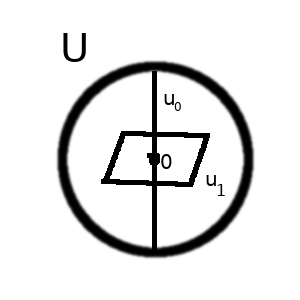
\includegraphics[width=\linewidth]{1.png}
		\caption{$U_0 = k + vA$}
	\end{subfigure}
	\begin{subfigure}[b]{0.25\linewidth}
		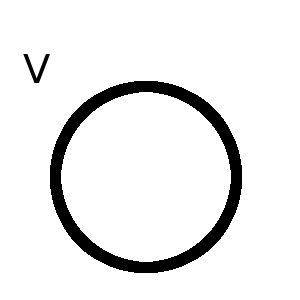
\includegraphics[width=\linewidth]{2.png}
		\caption{$U = U_0 \oplus U_1$}
	\end{subfigure}
	\begin{subfigure}[b]{0.25\linewidth}
		\caption{$U_1 \cap U_1 = \{0\}$}
	\end{subfigure}
\end{figure}
$\forall v \in U\ u = u_0 + v_1$ единственным образом \newline
$A u = A \underset{Ker A}{\underbrace{u_0}} + A u_1 = A u_1$. Значит $Im a = A V_1$ \newline
$A_1 = A|_{u_1}: u_1 \rightarrow Im A$, $A_1$ - изоморфизм. \newline
$U_1 \cong Im A \Leftrightarrow dim(U_1) = dim(Im\ a) \Leftrightarrow dim(Ker A) \neq dim(Im\ a) = dim(U)$ \newline
\bfline{Следствия}:
\begin{enumerate}
	\item $A \in L(U, V)$ эквивалентно:
		\begin{enumerate}
			\item $A$ --- изоморфизм
			\item $dim V = dim U = rg A$
			\item $dim U = dim V$, $Ker A = \{0\}$
		\end{enumerate}
	\item $A \in End(V)$ эквивалентно
		\begin{enumerate}
			\item $A$ --- изоморфизм
			\item $dim V = rg A$
			\item $Ker A = \{0\}$
		\end{enumerate}
\end{enumerate}
\end{document}